\section{Supplementary design, analysis, and reproducibility details}
\label{app:supplement}

\subsection{Case construction and balance}

The medical tasks use the checked-in canonical evidence schema shared with the human website. Legal cases were grounded in the NYC OATH Hearings Division dataset and public hearing guidance; financial cases were constructed from source facts together with the CFPB Consumer Complaint Database and Regulation E error-resolution guidance. These labels are fixed study references for analysis. CFPB company-response categories are not treated as normative ground truth, and independent domain experts will review nonmedical action boundaries before a human extension.

\begin{table}[h]
\centering
\caption{Case balance in the expanded cross-domain simulation.}
\small
\begin{tabular}{lrrrr}
\toprule
Domain & Cases & Lower reference & Higher reference & Trials\\
\midrule
Medical & 10 & 5 & 5 & 160\\
Legal & 10 & 5 & 5 & 160\\
Finance & 10 & 5 & 5 & 160\\
\bottomrule
\end{tabular}
\end{table}

The sandbox used MatrAIx pinned to commit \texttt{ea16f1} with GPT-4.1-mini as the persona-agent backbone. The manifest contains 480 full-probe trials: 120 definition-identical records reused from the preceding case-expansion run and 360 newly executed records for three additional personas. Each of four personas contributes 120 trials, with ten cases in every domain and every formal Direction $\times$ Confidence cell complete. We excluded a preliminary run that omitted case context before the first action and allowed automatic evidence reveal.

\subsection{Probe schedule, features, and grouped prediction}

All 480 trials used the full-probe schedule so every completed interaction cycle had a corresponding evaluation label. Each probe was a stateless call to the same backbone and persona prompt, with access to the opening problem and visible dialogue through that turn. Probe outputs were stored outside the visible dialogue, were not appended to subsequent persona context, and were unavailable to the advising model. The run therefore does not estimate probe reactivity from the act of elicitation, although probe text did not directly condition later actions. Because the evaluator observed the visible history, its reports can reflect interaction information also represented in behavioral features; observability therefore measures predictive correspondence with elicited reports rather than independent validation of latent internal states. Probe values changed within trials: the proportion of adjacent nonzero changes was .406 for urgency, .564 for information need, .561 for intended action, and .583 for uncertainty.

The context feature set comprised case ID, domain, turn, AI recommendation escalation, and AI confidence. Observable features comprised message length and question indicators; current and cumulative information actions; structured and conversational canonical evidence IDs; number acquired and remaining; current and cumulative timing; and continuation/stopping. Current and previous self-reported states were excluded. Categorical variables were one-hot encoded within each training fold, continuous predictors were standardized within fold, and ridge regularization was selected using training data only.

Each of four folds held out one persona. Predictions from all held-out folds were concatenated before computing $R^2$. Behavior-only grouped-CV $R^2$ was .047, .461, .012, and .093 for urgency, information need, action, and uncertainty, respectively. The primary comparison retained context in both models because a behavior-only score cannot distinguish a behavioral signature from case composition or policy assignment.

\subsection{Domain, modality, and corruption analyses}

Domain-specific context/context-plus-behavior $R^2$ for information need was .611/.700 in medicine, .441/.513 in law, and .516/.575 in finance, giving increments .089, .071, and .059. These fits use within-domain grouped-by-persona prediction. The pooled estimator includes domain as context and is not a leave-domain-out analysis.

Modality ablations evaluated full behavior, no text, text only, information actions only, continue/stop only, evidence trajectory only, and timing only. Corruption tests modified observable behavior while leaving probe labels and context intact: event dropout at 10\%, 20\%, and 40\%; removal of information actions; no text; text only; text truncation; timing removal; sparse logs; and combined moderate noise. Fixed seed 20260812 was used. These tests characterize sensitivity to controlled degradation, not selective real-world missingness.

\subsection{Dynamic transition analysis}

The V8 transition analysis aligned each pre-turn state with its subsequent post-turn state, yielding 2,362 transitions. Standardized state changes were regressed on pre-turn state, AI recommendation escalation, AI confidence, their interaction, observed action and evidence features, task reference, turn, domain, and persona indicators. Standard errors were clustered by persona. This specification describes conditional updating under the implemented policy rather than an optimal policy, utility function, or mediation mechanism.

Higher AI recommendations predicted upward intended-action updating ($\beta=.510$). High AI confidence predicted reduced information need ($\beta=-.316$) and uncertainty ($\beta=-.855$). Distance to the AI-advised action fell more strongly ($\beta=-.317$ for higher recommendations) than distance to the fixed task reference ($\beta=-.048$). Supplementary Figures~\ref{fig:v8-trajectories}--\ref{fig:v8-policy} visualize self-reported-state trajectories, transition coefficients, and the separation between AI-advice and task-reference convergence.

\begin{figure}[t]
  \centering
  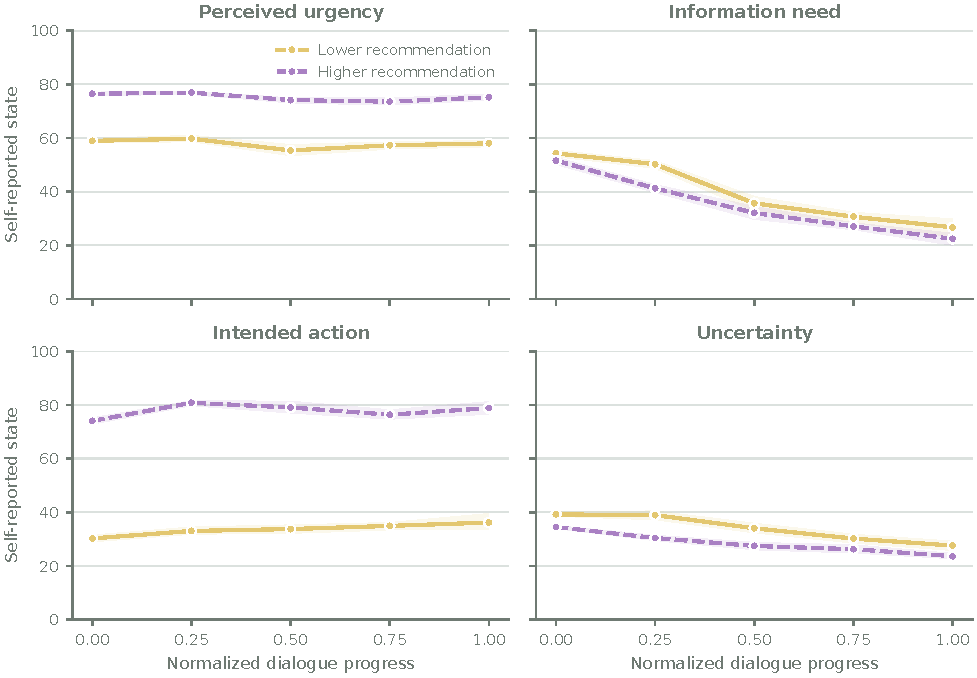
\includegraphics[width=\linewidth]{figs/v8_state_trajectories.pdf}
  \caption{Simulated-user self-reported-state trajectories. Means show how the four states evolve across completed dialogue cycles in the V8 transition dataset.}
  \label{fig:v8-trajectories}
\end{figure}

\begin{figure}[t]
  \centering
  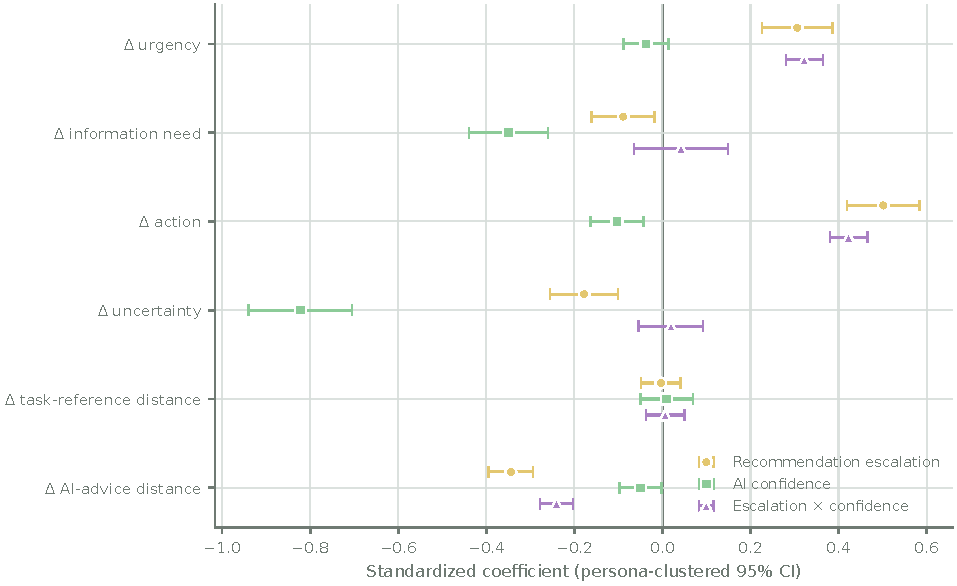
\includegraphics[width=\linewidth]{figs/v8_ai_influence_forest.pdf}
  \caption{Conditional transition coefficients. The forest plot reports standardized associations between experimental inputs and within-dialogue updating. Intervals use persona-clustered standard errors and should be interpreted with four persona clusters.}
  \label{fig:v8-forest}
\end{figure}

\begin{figure}[t]
  \centering
  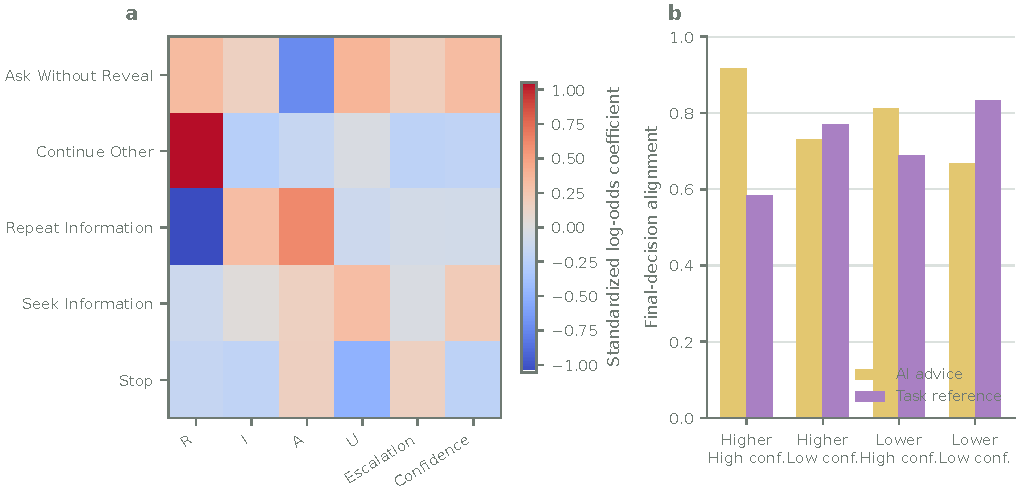
\includegraphics[width=\linewidth]{figs/v8_policy_and_final_decision.pdf}
  \caption{Advice responsiveness versus task-reference convergence. The panels distinguish movement toward the AI-advised endpoint from movement toward the fixed case reference.}
  \label{fig:v8-policy}
\end{figure}

\subsection{Human-freeze audit}

The main text reports the 109 completed participant records in the 2026-09-03 backup. They contain 218 completed case trajectories and 941 state ratings: 184 baseline and 757 post-turn reports. After chronological reindexing, 159 trajectories contain at least one post-turn probe. Qualtrics randomized the AI-assisted versus human-reasoning condition. Within AI-assisted sessions, recommendation level and AI confidence were balanced at session creation and fixed before interaction. A recommendation-bearing statement appeared in every returned assistant response, so delivered exposure required a participant message and response. Eighty-two case trajectories meet that exposure definition; 46 are viral-gastroenteritis trajectories forming the four-cell comparison (cell sizes 14, 11, 12, and 9 for lower/low, lower/high, higher/low, and higher/high). Recommendation analyses condition on delivered case-level exposure and are descriptive; delivered exposure itself was not independently randomized.

The raw UI payload counter restarted within otherwise continuous case histories. The analysis retains every rating, sorts events by timestamp, assigns baseline to turn 0, and renumbers post-turn ratings sequentially within participant and case. The original payload index is retained as \texttt{logged\_turn\_index} for audit. This prevents different chronological cycles from being collapsed into the same plotted turn. Human turn-level counts after correction are 159, 147, 142, 130, 93, 43, 20, 8, 5, 4, 3, 2, and 1 for turns 1--13 across cases; case-specific counts are reported in the reproducibility export.

Across the 82 recommendation-exposed trajectories, the median case-level mean assistant latency was 10.39 seconds (range 3.11--21.78; 432 responses). The question-mark metric is literal punctuation, not a semantic question-act classifier. It remains in the exported audit table but is not plotted as a substantive measure of information seeking.

\begin{figure}[t]
  \centering
  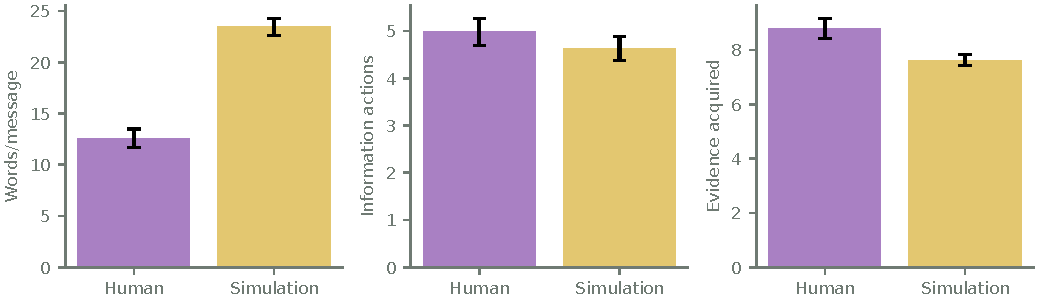
\includegraphics[width=\linewidth]{figs/human_simulation_conversation_comparison.pdf}
  \caption{Observable channels in matched viral gastroenteritis. Means and SEM across 46 recommendation-exposed human and 16 simulated trajectories. Message length differs substantially, while information actions and canonical evidence acquisition are closer in scale.}
  \label{fig:human-conversation}
\end{figure}

\subsection{Prespecified final-freeze human inference}

The final human analysis will fit context-only and context-plus-behavior ridge models using leave-one-participant-out prediction. The primary statistic is $\Delta R^2_{I,\mathrm{human}}$; the same statistic will be reported for urgency, action, and uncertainty. Information need is the prespecified confirmatory target, and the other states are secondary. Raw one-sided p-values and Holm--Bonferroni-adjusted p-values across all four states will be reported.

Because participant clusters have unequal trajectory lengths and cross-validated $\Delta R^2$ has no simple parametric null, inference will use participant-level randomization. Each permutation preserves a participant's context--probe pairs and reassigns complete behavioral sequences only among donors with the same case. Sequences are aligned chronologically; after a donor sequence stops, current-turn actions remain absent and cumulative evidence is carried forward. LOPO models will be refit for 5,000 Monte Carlo permutations (seed 20260812), with a plus-one-corrected one-sided p-value.

Magnitude uncertainty will use 5,000 participant-cluster bootstrap resamples (seed 20260813), sampling participants with all their eligible cases and turns and refitting the LOPO contrast. Percentile 95\% intervals will describe precision. These procedures will be run once at the final data freeze. Interim backups are used for descriptive trajectory and exposure audits only, which avoids optional stopping while recruitment is active.

\subsection{Reproducibility and release boundary}

Simulation code, task definitions, configuration, persona-grouped splits, analysis scripts, and derived nonhuman artifacts are prepared for public release. Human release materials contain only approved aggregated or de-identified fields and follow the consent and protocol restrictions. Private paths, credentials, SONA tokens, linkage secrets, and API keys are excluded. The analysis script preserves raw logged turn indices alongside corrected chronological indices, writes per-turn sample counts, and generates the manuscript figures from exported tables. The release URL is pending final repository publication.
